\documentclass[tikz,border=2pt,11pt]{standalone}
\usetikzlibrary{arrows.meta}
\usetikzlibrary{decorations.pathreplacing}
\usetikzlibrary{calc}
\usetikzlibrary{positioning}
\usepackage{amsmath}
\usepackage{amssymb}
\usepackage{graphicx}
\usepackage{xcolor}
\usepackage{tikz}
\newcommand{\R}{\mathbb R}
\newcommand{\C}{\mathbb C}
\newcommand{\Z}{\mathbb Z}
\newcommand{\Q}{\mathbb Q}
\newcommand{\F}{\mathbb F}
\newcommand{\CP}{\mathbb{CP}}
\newcommand{\RP}{\mathbb{RP}}
\newcommand{\SU}{\operatorname{SU}}
\newcommand{\U}{\operatorname{U}}
\newcommand{\SO}{\operatorname{SO}}
\newcommand{\PU}{\operatorname{PU}}
\newcommand{\Spinc}{\operatorname{Spin}^{c}}
\newcommand{\PD}{\operatorname{PD}}
\newcommand{\id}{\operatorname{id}}
\newcommand{\ad}{\operatorname{ad}}
\newcommand{\tr}{\operatorname{tr}}
\newcommand{\ind}{\operatorname{ind}}
\newcommand{\coker}{\operatorname{coker}}
\newcommand{\Hol}{\operatorname{Hol}}
\newcommand{\Scal}{\operatorname{Scal}}
\newcommand{\Vol}{\operatorname{Vol}}
\newcommand{\supp}{\operatorname{supp}}
\newcommand{\im}{\operatorname{im}}
\newcommand{\diag}{\operatorname{diag}}
\newcommand{\Hom}{\operatorname{Hom}}
\newcommand{\End}{\operatorname{End}}
\newcommand{\dist}{\operatorname{dist}}
\newcommand{\rank}{\operatorname{rank}}
\newcommand{\codim}{\operatorname{codim}}
\newcommand{\Sym}{\operatorname{Sym}}
\newcommand{\GL}{\operatorname{GL}}
\newcommand{\grad}{\operatorname{grad}}
\begin{document}
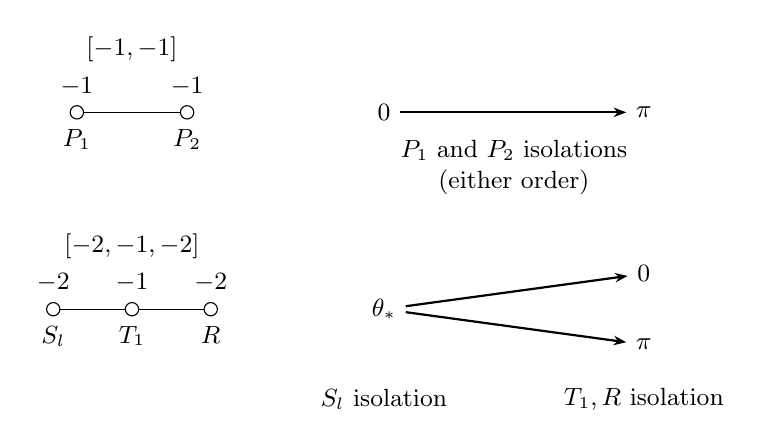
\begin{tikzpicture}[font=\small,
 sphere/.style={circle,draw,inner sep=1.7pt},
 path/.style={-{Stealth[length=1.6mm]},thick}]
 \node at (1,1.9) {$[-1,-1]$};
 \node[sphere,label=above:$-1$,label=below:$P_1$] (p1) at (0.3,1.1) {};
 \node[sphere,label=above:$-1$,label=below:$P_2$] (p2) at (1.7,1.1) {};
 \draw (p1)--(p2);
 \node (zero) at (4.2,1.1) {$0$};
 \node (pi) at (7.5,1.1) {$\pi$};
 \draw[path] (zero)--(pi);
 \node[align=center] at (5.85,0.4) {$P_1$ and $P_2$ isolations\\(either order)};
 \node at (1,-0.6) {$[-2,-1,-2]$};
 \node[sphere,label=above:$-2$,label=below:$S_l$] (sl) at (0,-1.4) {};
 \node[sphere,label=above:$-1$,label=below:$T_1$] (t1) at (1,-1.4) {};
 \node[sphere,label=above:$-2$,label=below:$R$] (r) at (2,-1.4) {};
 \draw (sl)--(t1)--(r);
 \node (common) at (4.2,-1.4) {$\theta_*$};
 \node (z0) at (7.5,-0.95) {$0$};
 \node (zpi) at (7.5,-1.85) {$\pi$};
 \draw[path] (common)--(z0);
 \draw[path] (common)--(zpi);
 \node[align=center] at (4.2,-2.55) {$S_l$ isolation};
 \node[align=center] at (7.5,-2.55) {$T_1,R$ isolation};
\end{tikzpicture}
\end{document}
